\documentclass[12pt,makeidx]{amsbook}

\usepackage[pdfauthor   = {Kamal Saleh},
            pdftitle    = {Test file},
            pdfsubject  = {},
%             pdfkeywords = {},
            bookmarks=true,
            bookmarksopen=true,
            pagebackref=true,
            hyperindex=true,
            colorlinks=true,
            linkcolor=blue,
            citecolor=blue,
            filecolor=blue,
            urlcolor=blue,
            ]{hyperref}

\usepackage[utf8]{inputenc}
\usepackage[T1]{fontenc}
\usepackage[english]{babel}
\usepackage{mathrsfs}
\usepackage{mathtools}
\usepackage{amssymb}
\usepackage{amsthm}
\usepackage{amsmath}
\usepackage[dvipsnames]{xcolor}
\usepackage{tikz}
\usepackage{tikz-cd}
\usetikzlibrary{automata,shapes,arrows,matrix,backgrounds,positioning,plotmarks,calc,patterns,matrix,decorations.pathreplacing,decorations.pathmorphing,decorations.text,decorations.markings}

\tikzset{
  mysquare/.style={
    draw,minimum size=1cm,align=center,
    append after command={node[fill,anchor=north west,minimum size=0.35cm] at (\tikzlastnode.north west) {}}
  },
  twoarrows/.style n args={4}{
    decoration={
      markings,
      mark=at position #1 with {\arrow{>}\node[above] {#3};}, 
      mark=at position #2 with {\arrow{>}\node[above] {#4};} 
    },
  postaction=decorate  
  },
  onearrow/.style 2 args={
    decoration={
      markings,
      mark=at position #1 with {\arrow{>}\node[above] {#2};}, 
    },
  postaction=decorate  
  },
  onearrowrev/.style 2 args={
    decoration={
      markings,
      mark=at position #1 with {\arrow{<}\node[above] {#2};}, 
    },
  postaction=decorate  
  },
}

\begin{document}
\begin{titlepage}
  \vspace*{\stretch{1.0}}
  \begin{center}
     \Large\textbf{Test file }
  \end{center}
  \vspace*{\stretch{2.0}}
\end{titlepage}

\begin{center}
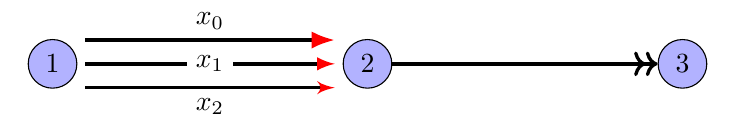
\begin{tikzpicture}[x=4cm,y=1.5cm,transform shape,
mylabel/.style={thick, draw=black, 
align=center, minimum width=0.5cm, minimum height=0.5cm,fill=white}]
\node[draw,shape=circle, fill=blue!30] (2V0) at (2,0) {$3$};
\node[draw,shape=circle, fill=blue!30] (1V0) at (1,0) {$2$};
\node[draw,shape=circle, fill=blue!30] (0V0) at (0,0) {$1$};
\draw [transform canvas={yshift=2ex},->,very thick,shorten >=0.1cm,shorten <=0.1cm, -{Latex[red]}] (0V0)-- node[above]{$x_0$} (1V0);
\draw [transform canvas={yshift=0ex},->,very thick,shorten >=0.1cm,shorten <=0.1cm, -{latex[red]}] (0V0)-- node[fill=white, anchor=center, pos=0.5,font=\bfseries]{$x_1$} (1V0);
\draw [transform canvas={yshift=-2ex},->,very thick,shorten >=0.1cm,shorten <=0.1cm, -{latex'[red]}] (0V0)-- node[below]{$x_2$} (1V0); % or (1,0);
\draw[->>,very thick] (1V0)-- (2V0);
\end{tikzpicture}
\end{center}

%paste here the tex code of the diagram
\end{document}
